\subsubsection{Site specifications}
	Need for geothermal district heating/cooling demand for potentially the entire campus. It is crucial to assess the possibilities of using deeper geothermal heat exchangers. 
\subsubsection{Boreohle Heat Exchanger}
	
\subsubsection{Experimental Setup}
	To characterise the thermal potentials of boreholes, thermal response tests (TRTs) are often used when estimating the borehole resistances. Following the ASHARE guidelines, the inlet and outlet temperature at the borehole are recorded. The thermal conductivity of the borehole is the mean rate of temperature change over the natural logarithmic time of either the inlet or outlet temperature beyond the initial period of heat injection. The thermal conductivities are further used to estimate the borehole resistance and other parameters to evaluate potential borehole field designs. This method clearly does not provide enough information regarding the temperature evolution along the depth of borehole, i.e. the geothermal gradient situation of individual boreholes. Recent research have pointed out possibilities to use distributed TRTs that utilise fibre optic sensors that produces depth-specific temperature measurement along the borehole.  
	
	The state-of-the-art methods used in estimating the thermal properties during thermal response tests (TRTs) were first proposed by Ingersol in 1954, and further expanded into ASHRAE guidelines in ASHRAE Handbooks. This method attempt to estimate the borehole resistance through three hypothetical stages of heat injection.  
	
	To estimate the thermal conductivity of the formation, a thermal response test was performed on the drill site on September 10th, 2019. The test follows the guidelines recommended by the Americal Society of Heating, Refrigeration and Air-Conditioning Engineers (ASHRAE) in its HVAC Applications Handbook, Geothermal Energy Chapter. The borehole was uniformed grouted from the bottom to the top via premie pipe, and had a delay of more than five days between loop installation and test startup. The undisturbed formation temperature was estimated through the recorded temperature from the fiber optic cable installed along and around the borehole heat exchanger. The duration of the test was 48.5 hours, where the data (inlet, outlet temperature and heat injection rates) was collected every five minutes.  The heat injected was estimated to be 51 to 85 Btu/hr (or 15 to 25 W) per foot of the borehole, which averaged to be approximately 30.5 kW total heat input throughout the test. 

	\begin{figure}
	\centering
	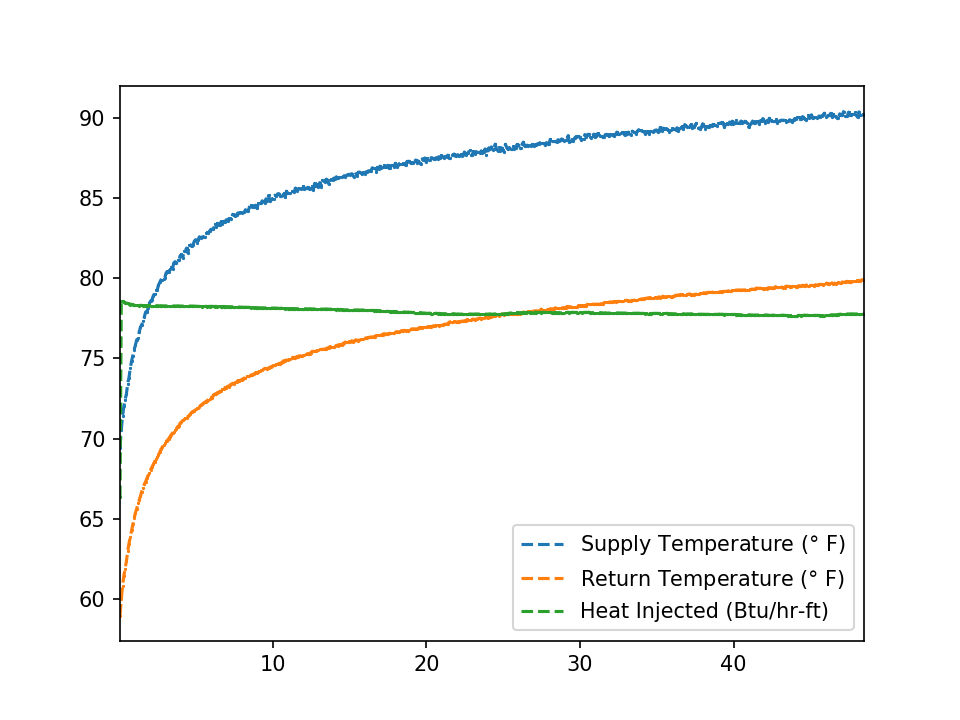
\includegraphics[width=0.5\textwidth]{data/TRTraw}	
	\caption{Temperature measured at the inlet and outlet of the well site.}\label{fg:raw}
	\end{figure}
	
	For the purpose of the conventional TRT the project procured, the data collected by the company performing the test first undergone the procedures of a conventional TRT calculation. The relatively steady slope shown in Figure~\ref{fg:raw} of both the inlet and outlet temperatures since the 10th hour of the operation can be used to determine the overall thermal conductivity of the borehole, and can be further expanded into the thermal diffusivity of the formation through an estimated heat capacity of the borehole. The overall borehole resistance may therefore be estimated through Equation. 
	
	\begin{equation}
		R_b = \frac{H}{Q}\{ T(t) - T_g -\frac{Q}{4\pi \lambda_g H} [E_i(\frac{r_b}{4 \alpha_g t})]   \}
	\end{equation}